\documentclass[10pt,a4paper]{article} 
\usepackage{times}
\usepackage{a4wide}
\usepackage{ukdate}
\usepackage{cite}
%\usepackage{epsfig}
\usepackage[pdftex]{graphicx}
\usepackage{harvard}
\usepackage{alltt}
\usepackage{pifont}
\usepackage{pslatex}

\title{SWARM 0.44 Documentation} 

\author{Michael Dales \\[2mm]
Department of Computing Science,
University of Glasgow,\\
\small{17 Lilybank Gardens,
Glasgow, G12 8RZ, Scotland.}\\
\small{michael@dcs.gla.ac.uk}\\
\small{Copyright 2000 \Pisymbol{psy}{227} Michael Dales}}
\date{}

\begin{document}
\bibliographystyle{agsm}
\citationmode{abbr}

\maketitle

%%%%%%%%%%%%%%%%%%%%%%%%%%%%%%%%%%%%%%%%%%%%%%%%%%%%%%%%%%%%%%%%%%%%%%%%%
\begin{abstract}
This document gives a brief explanation of the design and
implementation of SWARM --- the Software ARM. It explains what SWARM
is, and what it isn't, along with the design philosophy.
\end{abstract}
%%%%%%%%%%%%%%%%%%%%%%%%%%%%%%%%%%%%%%%%%%%%%%%%%%%%%%%%%%%%%%%%%%%%%%%%%

%%%%%%%%%%%%%%%%%%%%%%%%%%
%%%%%%%%%%%%%%%%%%%%%%%%%%
\section{Introduction} %%%
\label{sec:intro}      %%%
%%%%%%%%%%%%%%%%%%%%%%%%%%
%%%%%%%%%%%%%%%%%%%%%%%%%%

The original idea behind SWARM was to design an ARM processor module
to plug into the SimOS system developed at Stanford
University. SimOS~\cite{rosenblum:sosp95} is a software simulator of
an entire computer, enough to run real operating systems and
applications, in order to easily benchmark changes to the
system. SimOS is based upon MIPS and Alpha processors. A research
project at the University of Glasgow required a complete machine
emulator for an ARM based system, so work began on SWARM. However, it
soon became apparent that the work in linking SWARM into SimOS was not
justified, and attempts to link the two projects were abandoned.

SWARM is now a stand alone software project. It comprises a set of C++
classes that allow emulation of various parts of an ARM processor. The
hierarchy allows users to use either the simple core, or a processor
with core and caches.

The aim of SWARM was never to simply run ARM binaries on another
platform, but rather to allow research into the modification of the
ARM datapath. Thus SWARM models the internal datapath of the ARM
core\footnote{The SWARM core is modelled on the ARM6 core. The rest of
the system is based \emph{very} loosely on a StrongARM.} and
instructions are decoded into a set of control signals to manipulate
the datapath. Another requirement for SWARM was that it provide
support for the full register/cache/external memory hierarchy. To this
end SWARM provides an abstract cache class which can have different
implementations, and also supports either Harvard or Princeton style
caches. 

%%%%%%%%%%%%%%%%%%%%%%%%%%%%%%%%
%%%%%%%%%%%%%%%%%%%%%%%%%%%%%%%%
\section{SWARM Architecture} %%%
\label{swarmarch}            %%%
%%%%%%%%%%%%%%%%%%%%%%%%%%%%%%%%
%%%%%%%%%%%%%%%%%%%%%%%%%%%%%%%%

%%%%%%%%%%%%%%%%%%%%%%%%%%%%%%%
\subsection{SWARM Datapath} %%%
\label{sec:datapath}        %%%
%%%%%%%%%%%%%%%%%%%%%%%%%%%%%%%

The datapath used in SWARM tries to honour that of the real datapath
as much as possible. A simplified version of the datapath can be found
in~\cite{furber:arm96}, but this does not include all the information
necessary. For instance, during load/store multiple commands magic
numbers need to appear on one of the buses. The datapath used inside
SWARM can be seen in Figure~\ref{fig:datapath}.

\begin{figure}
\centering
%\mbox{\epsfig{file=pics/arm6blk.eps,height=8cm}}
\mbox{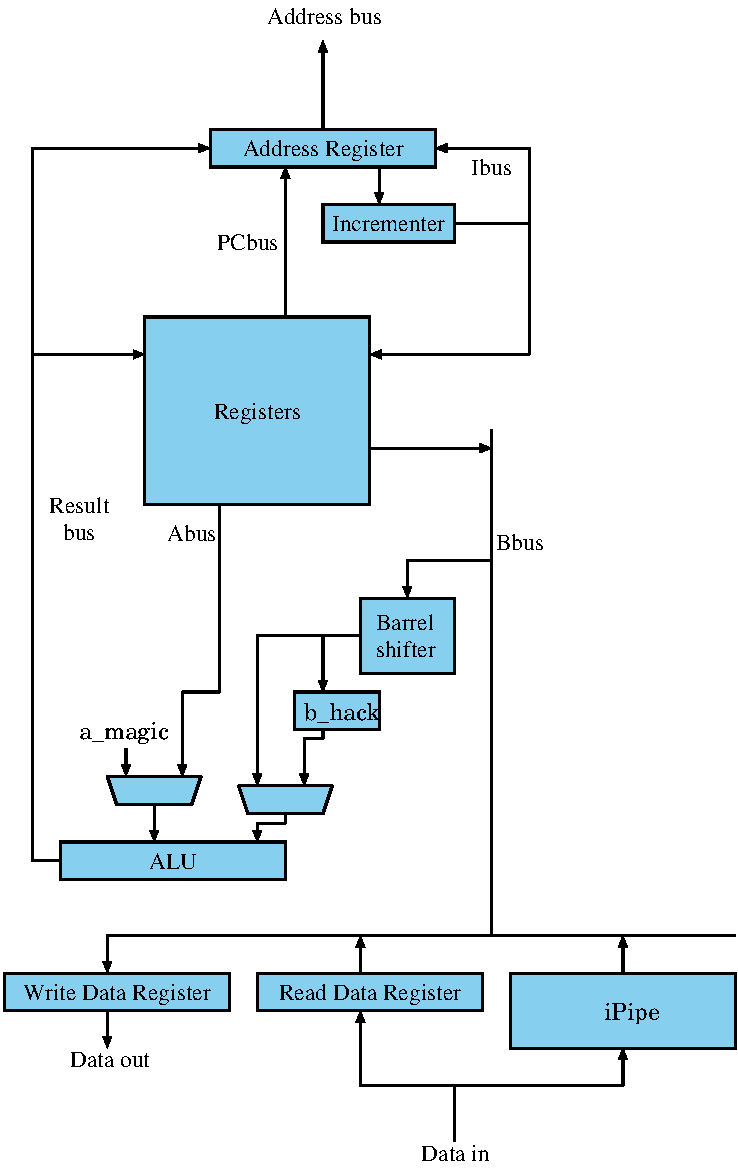
\includegraphics[height=8cm]{pics/arm6blk}}
\caption{SWARM datapath.}
\label{fig:datapath}
\end{figure}

The datapath looks as you would expect it: the register file in the
centre, the ALU fed by the A bus and the output of the B bus passed
through a barrel shifter. Then there are the registers and the
instruction pipe (the instruction pipe contains the current
instruction and the next instruction in the pipeline). However, there
are also two notable additions. The \emph{b\_hack} register contains
the last value on the B input to the ALU, and \emph{a\_magic} is a
magic number. The delay register on the B path is needed to allow
load/store writeback calculations to occur without needing an extra
cycle while the B bus is in use. The magic value on the A input to the
ALU is used to generate offsets during load/store multiple
instructions.


%%%%%%%%%%%%%%%%%%%%%%%%%%%%%%%%%
\subsection{Memory Hierarchy} %%%
\label{sec:memory}            %%%
%%%%%%%%%%%%%%%%%%%%%%%%%%%%%%%%%

SWARM attempts to realistically model the memory hierarchy for a
simple ARM machine. This was originally necessary due to the intended
purpose of SWARM, but turned out to make for a nice way of making the
memory interaction simpler to implement. SWARM does not,
unfortunately, implement a full realistic external memory bus. 
Currently the ARM processor interface simply provides 32 bit addresses
and data values. This was simple to implement and met the
requirements for the project. Memory is provided as a large array of
\texttt{char} types.

The memory access process can be split into three parts: ARM core
interface, the ARM processor interface (which includes the cache), and
the main memory itself. The cache is an integral part of the
system. If there is a cache miss on a read then the ARM processor
halts the core, fetches the data from memory into the cache and then
continues the execution of the core. As far as the core was concerned
the data was in the cache.
To help you understand the way control flows between the three within
the emulator see the rough timing diagrams in Figure~\ref{fig:memory}. 

\begin{figure}
\centering
%\mbox{\epsfig{file=pics/mem.eps,height=4cm}}
\mbox{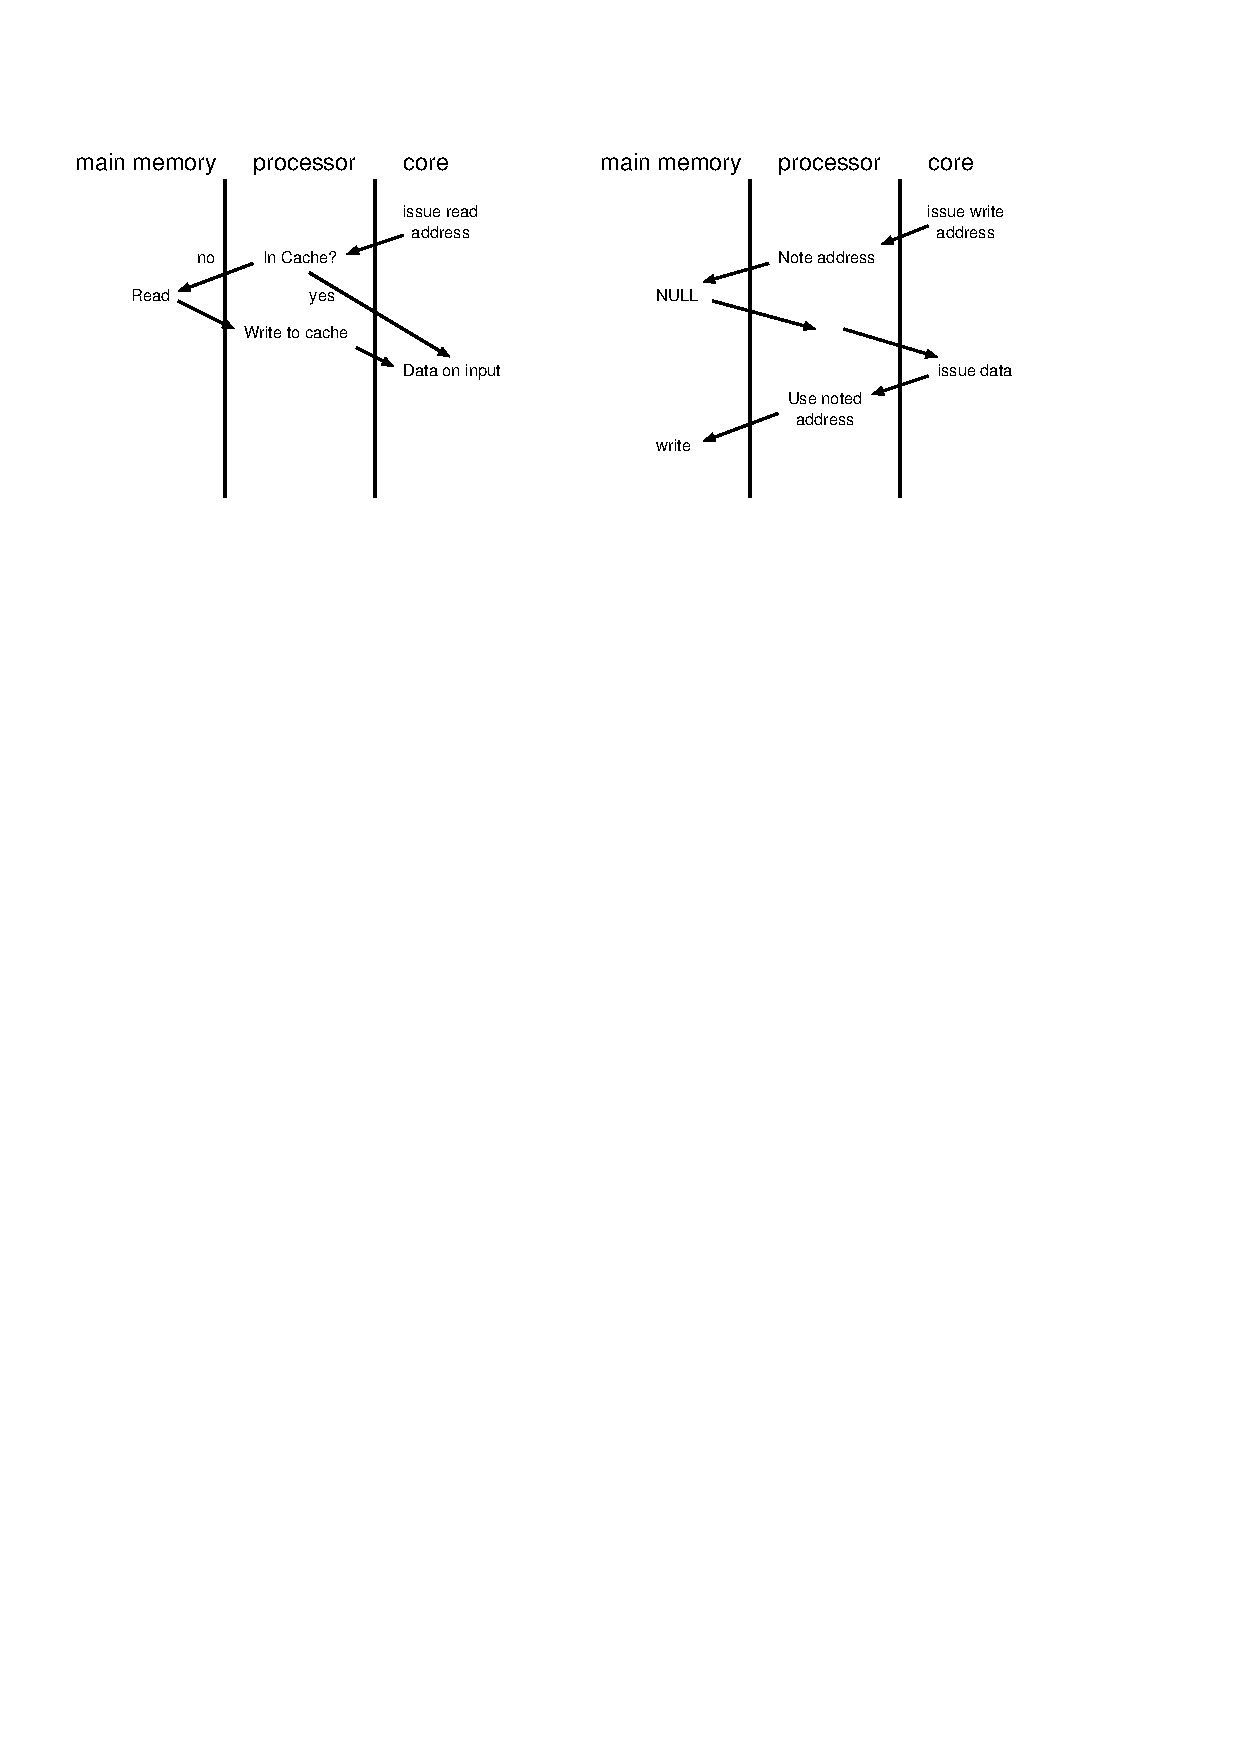
\includegraphics[height=4cm]{pics/mem}}
\caption{SWARM memory accesses: 1) Read 2) Write.}
\label{fig:memory}
\end{figure}


%%%%%%%%%%%%%%%%%%%%%%%%%%%%%
\subsection{Coprocessors} %%%
\label{sec:copro}         %%%
%%%%%%%%%%%%%%%%%%%%%%%%%%%%%

Currently a small amount of support for internal coprocessors is
enabled in SWARM. Implemented is a very basic system coprocessor. This
is currently only used to provide a chip type ID and for accessing the
cycle counter from software running on SWARM (see
\texttt{libc/include/profile.h} to see how this is done). 


%%%%%%%%%%%%%%%%%%%%%%%%%%%%%%%%%%%%%%%%%%%%%%%%%%%%%%%%%
\subsection{Communicating between ARM code and SWARM} %%%
\label{sec:comms}                                     %%% 
%%%%%%%%%%%%%%%%%%%%%%%%%%%%%%%%%%%%%%%%%%%%%%%%%%%%%%%%%            

It is useful to allow applications executing on SWARM to be able to
invoke sections of code in SWARM (for example, asking SWARM to halt at
the end of a program). This is done through the Software
Interrupt (SWI) mechanism. A
SWI call takes a 24 bit constant as its parameter. This space has
been divided into two parts. All SWI calls where the top bit of the
constant is zero are handled as would be expected on a real ARM and
call emulated code via the SWI vector. However, if the top bit is set
to one then the call is emulated as a no-op, and at the same time a
function in SWARM can be called. 

Functions invoked this way mimic the standard ARM procedure call
convention. They take four unsigned integers which receive the first
for register values, and will return an unsigned integer which is
placed in register zero after the call.
See the code for examples of how this works.



%%%%%%%%%%%%%%%%%%%%%%%%%%%%%%%
%%%%%%%%%%%%%%%%%%%%%%%%%%%%%%%
\section{SWARM Source Core} %%%
\label{sec:code}            %%%
%%%%%%%%%%%%%%%%%%%%%%%%%%%%%%%
%%%%%%%%%%%%%%%%%%%%%%%%%%%%%%%

%%%%%%%%%%%%%%%%%%%%%%%%%%%%%%
\subsection{Code Overview} %%%
\label{sec:overview}       %%%
%%%%%%%%%%%%%%%%%%%%%%%%%%%%%%

Here is a quick tour of the main classes in SWARM. More detailed
explanations will follow as necessary. 

\begin{itemize}
\itemsep 0pt
\parsep 0pt

\item \textbf{CArmCore} (core.cpp/core.h/alu.cpp/alu.h) --- This class
handles the ARM core; that is the datapath as described in
Section~\ref{sec:datapath}. Communicates using a bus structure based
on the ARM6 core pin--out. 

\item \textbf{CArmProc} (armproc.cpp/armproc.h) --- CArmProc provides
a processor view. It includes the caches and is responsible for
managing the memory hierarchy. 

\item \textbf{CCache} (cache.cpp/cache.h) --- Provides an abstract
interface for a cache. Reports cache misses using exceptions.

\item \textbf{CDirectCache} (direct.cpp/direct.h) --- Implements a
direct mapped cache.

\item \textbf{CAssociativeCache} (associative.cpp/associative.h) ---
Implements a fully associative cache.

\end{itemize}

The main program at the moment is very simple. Its sole purpose is to
provide a simple test harness for SWARM. Currently the test harness
requires an ARM binary to be provided as the only parameter. This
binary image is loaded into the emulated system's memory, and
execution starts from address zero.


%%%%%%%%%%%%%%%%%%%%%%%%%
\subsection{CArmCore} %%%
\label{sec:carmcore}  %%%
%%%%%%%%%%%%%%%%%%%%%%%%%

CArmCore is where all the interesting bits happen. All the state for
the datapath is stored as member variables in the class. For each
each instruction the decode stage will generate a series of control
information structures (on for each cycle the instruction will take)
which are applied to the datapath on the Exec method call. The
structure type CONTROL contains all the information for managing the
datapath and how it interfaces with the bus between the core and the
rest of the world.

The user interacts with the core using the Cycle method - this clocks
the datapath and causes all the registers to updates. The Cycle method
takes a structure of type CBIOTAG which mimics the pin--out of the ARM
core. Not all the fields are currently used (see comments in core.h).

%%%%%%%%%%%%%%%%%%%%%%%%%
\subsection{CArmProc} %%%
\label{sec:armproc}   %%%
%%%%%%%%%%%%%%%%%%%%%%%%%

This class approximates the system on chip view of an ARM - it 
basically acts as
glue between the external interface, the caches, and the core. The
interesting stuff here happens in the Cycle method. This is the method
that users of the class should call to make things happen. The
workings here are like a state machine with transitions happening on
every invocation. This can be seen in Figure~\ref{fig:state}. In
normal operation instructions and data are read from the cache and
processed. If there is a cache miss then the core is effectively
stalled as the cache line is filled, then execution continues as if
the cache hit had been successful. On a write we note the address
generated in the previous instruction and write the data generated in
the current instruction until a read operation occurs.

The type of cache used is defined by the preprocessor define
\texttt{CACHE\_TYPE}. This should be set to the name of a cache
implementation class. By default this is CDirectCache.

\begin{figure}
\centering
%\mbox{
\epsfig{file=pics/state.eps,height=4cm}}
\mbox{
\includegraphics[height=4cm]{pics/state}}
\caption{State machine of processor model}.
\label{fig:state}
\end{figure}

Look here to find the OS timer and interrupt controller. These are
modelled on those found in the Intel SA--1110 (see the SA--1110 manual
for a description on how they work).

%%%%%%%%%%%%%%%%%%%%%%%
\subsection{Status} %%%
\label{sec:status}  %%%
%%%%%%%%%%%%%%%%%%%%%%%

Currently there is enough of the ARM instruction set implemented to
allow simple programs to be compiled up in gcc and executed on
SWARM. The conditional execution works for all instructions, and the
following instruction classes have been implemented:

\begin{itemize}
\itemsep 0pt
\parsep 0pt
\item SWI calls.
\item Branch with and without link.
\item Data processing instructions.
\item 32 bit multiply with and without accumulate.
\item Single word/unsigned byte data transfer.
\item Load/store multiple.
\item Coprocessor register transfer instructions.
\item Reading and writing to the CPSR/SPSR.
\end{itemize}

SWARM has been tested on the following configurations:

\begin{itemize}
\itemsep 0pt
\parsep 0pt
\item G++ on ix86 and Alpha RedHat Linux systems.
\item Compaq C++ compiler for Alpha Linux.
\item Microsoft Developer Studio version 6.0.
\end{itemize}

The Microsoft Developer Studio workspace can be found in the MSVC
directory\footnote{My MSVC machine has gone temporarily, so these may
be a little out of date.}. The default make target is the gnu C++
compiler. The Compaq
C++ compiler can be used by passing the option \texttt{alpha-cxx}
parameter to make. 

%%%%%%%%%%%%%%%%%%%%%%%%%
%%%%%%%%%%%%%%%%%%%%%%%%%
\section{Using SWARM} %%%
\label{sec:using}     %%%
%%%%%%%%%%%%%%%%%%%%%%%%%
%%%%%%%%%%%%%%%%%%%%%%%%%

%%%%%%%%%%%%%%%%%%%%%%%%%%%%%%%%%%%%
\subsection{Compiling for SWARM} %%%
\label{sec:compiling}            %%%
%%%%%%%%%%%%%%%%%%%%%%%%%%%%%%%%%%%%

Currently the only supported technique for producing ARM binaries for
SWARM is using a gcc ARM compiler. On the author's system gcc was
built to produce binaries for \texttt{arm-unknown-coff}. The technique
is not just as simple as compiling and linking though. The binaries
that gcc produces have symbol information that SWARM will not
understand (unless you want to write an OS to run on top of SWARM to
load your binaries...). The overall procedure is:

\begin{enumerate}
\item Compile .c and .S files to .o files.
\item Do a preliminary link of binary. 
\item Find size of text, data, and bss sizes.
\item Link a new binary, with text, data, and bss sections packed
together.
\item Use objcopy to create a pure binary (i.e. no symbol information)
\end{enumerate}

The output of these steps is a raw ARM binary that can be executed on
SWARM. In the test apps directory it have a look at the make file used
to see the specifics of this operation.

Applications compiled using gcc require to be linked against a library
that provides functions called \texttt{\_\_\_gccmain} and
\texttt{\_start}. In addition we need to place the correct branches
into the first 6 (or 7 if you're not implementing FIQ properly) memory
addresses. To this end, \texttt{vector.S} contains the vector table,
and should be the first code in a binary image. Next comes crt0.S
which contains the \texttt{\_start} code. This is jumped to from the
reset vector. Unlike previous releases of SWARM,
\texttt{\_\_\_gccmain} is now brought in from the standard gcc
libraries (and does nothing).

There is a minimal C library implementation. This works in two
halves. Part of the system is implemented ``natively'' in ARM
assembler and has been taken from the NetBSD 1.4.1 release. More
complex parts (like those that implement I/O) have been implemented
using SWI
calls the emulator which has wrappers to the C library it is
linked against. The idea is that as much as possible should run
emulated on the ARM to provide more realistic profiling figures.


%%%%%%%%%%%%%%%%%%%%%%%%%%%%%%%%%%
\subsection{Test Applications} %%%
\label{sec:testapps}           %%%
%%%%%%%%%%%%%%%%%%%%%%%%%%%%%%%%%%

In the test apps directory are (currently) three test
applications. There are not particularly large applications, more
tests that have been added as SWARM grew in functionality. The simpler
tests remain for regression testing.

\begin{itemize}
\itemsep 0pt
\parsep 0pt

\item \textbf{test1} --- Simple program to calculate the first 10
Fibonacci numbers.
\item \textbf{test2} --- Program that duplicates a BMP file. It uses a
combination of the BSD libc memcpy and actual byte by byte transfers.
\item \textbf{test3} --- Simple test for memcpy.
\item \textbf{test4} --- Simple test for printf and stdio.
\item \textbf{filter} --- Program that runs an image through a sharpen
filter. Uses dynamic memory allocation.
\item \textbf{dumptest} --- Demonstrates both coprocessor data
transfers and the \texttt{\_dump} call to get SWARM to do a debug
dump.
\item \textbf{cpsrtest} --- Demonstrates the ability to read and write
to the CPSR and SPSR.
\item \textbf{timertest} --- Demonstrates the use of the OSTimer and
interrupt controller to generate events.
\end{itemize}

More meaningful examples may appear over time. The main limitation is
the lack of libc implementation, and of course, time.

%%%%%%%%%%%%%%%%%%%%%%%%%%
\subsection{Utilities} %%%
\label{sec:util}       %%%
%%%%%%%%%%%%%%%%%%%%%%%%%%

Swarm comes with some additional utilities. These can be found in the
bin directory at the top of the SWARM tree. Inside are:

\begin{itemize}
\itemsep 0pt
\parsep 0pt

\item \textbf{size.pl} --- This is a wrapper for the gcc size
utility. It is used by the make file in the test apps directory. 
\item \textbf{memcheck.pl} --- If you compile SWARM with
\texttt{-DDEBUG\_MEM} then SWARM will display all memory
allocations/deallocations in core.cpp. This Perl script will check
this output for anything that is not being freed up.
\item \textbf{arch} --- This is a wrapper script for Unix systems. It
returns information on processor type, OS type, and OS version. It is
used by the make files to guess the architecture type. This arch
script is Copyright 2000 \Pisymbol{psy}{227} University of Cambridge Computer Laboratory. It is
distributed with SWARM with their consent.
\item \textbf{disarm} --- Disarm will take a raw ARM binary and
convert it into ARM assembly. Useful as objdump won't work on the raw
binaries produced for SWARM.
\end{itemize}



%%%%%%%%%%%%%%%%%%%%%%%
%%%%%%%%%%%%%%%%%%%%%%%
\section{Todo List and Maintainance} %%%
\label{sec:todo}    %%%
%%%%%%%%%%%%%%%%%%%%%%%
%%%%%%%%%%%%%%%%%%%%%%%

There is a lot still to do. The main contenders are:

\begin{itemize}
\itemsep 0pt
\parsep 0pt
\item \textbf{Integrated Disarm} --- The observant may notice that
parts of disarm are in SWARM but commented out. In verbose mode SWARM
would spit out not only register information, but also the current 
instruction in human readable form. However support for this is
incomplete at time of writing, so this has been deactivated. Expect
this to appear in a near release.
\item \textbf{Documentation} --- Obviously.
\end{itemize}

If you are have an improvement for SWARM then feel free to mail it to
me and I'll test your submission and more than likely include it with
SWARM. Submissions should be in the form of patch files that I can
apply to the source (you can get diff for platforms other than Unix,
so being a non--Unix person is no excuse). If you \emph{really} can't send
me a patch, then send me as little source as possible and clearly
highlight what you have changed.

There is no CVS repository on--line. I doubt demand is that great for
updates, so SWARM will simply be provided as a tar--ball on the
web. If the demand is such then I am willing to move SWARM onto a
service such as Source Forge, but for the time being the distribution
mechanism will be kept as simple as possible. Announcements on
important new versions of SWARM could be posted to comp.sys.arm if
nobody there has any objections.

Bug reports should be e--mailed to me at the address given at the
start of this document.


%%%%%%%%%%%%%%%%%%%%%%%%%%%%%%
%%%%%%%%%%%%%%%%%%%%%%%%%%%%%%
\section{Acknowledgements} %%%
\label{sec:acks}           %%%
%%%%%%%%%%%%%%%%%%%%%%%%%%%%%%
%%%%%%%%%%%%%%%%%%%%%%%%%%%%%%

SWARM was originally produced as part of the author's PhD work at the
Department of Computing Science at the University of Glasgow. More
information on this work can be found at:
\newline
\newline
\texttt{http://www.dcs.gla.ac.uk/\Pisymbol{psy}{126}michael/phd/}. 
\newline
\newline
Additional technical information on the workings of the ARM processor
were provided by Dr. Richard Black. The research is funded by the
Engineering and Physical Sciences Research Council (EPSRC) and Xilinx, Inc.

%%%%%%%%%%%%%%%%%%%%%%%%%%%%%%%%%%%%%%%%%%%%%%%%%%%%%%%%%%%%%%%%%%%%%%%%%
\bibliography{swarm}

\end{document}
